\documentclass[a4paper,12pt,twoside,openright]{report}

\usepackage[utf8]{inputenc}
\usepackage[italian]{babel}
\usepackage[T1]{fontenc}
\usepackage[backend=biber,sorting=none]{biblatex}
\usepackage{amsmath}
\usepackage{blindtext}
\usepackage{color}
\usepackage{csquotes}
\usepackage{fancyhdr}
\usepackage{geometry}
\usepackage{graphicx}
\usepackage{lipsum}
\usepackage{listings}
\usepackage{pdfpages}
\usepackage{textcomp}
\usepackage{titlesec}

% ==== MARINGS, PARAGRAPHS, LINESPACE, TABLES, ETC. ====
\geometry{margin=3cm}
\setlength{\parskip}{0.7em}
\renewcommand{\baselinestretch}{1.5}

% ==== PAGE STYLING ====
\pagestyle{fancy}
\fancyhead{}
\fancyfoot[CE,CO]{}
\fancyfoot[LE,RO]{\thepage}

\definecolor{gray75}{gray}{0.75}
\newcommand{\PRLsep}{\noindent\makebox[\linewidth]{\resizebox{\linewidth}{1.5pt}{\textcolor{gray75}{$\bullet$}}}}
\renewcommand{\headrulewidth}{0pt}
\titleformat{\chapter}[hang]{\centering\Huge\bfseries}{\thechapter.\hspace{10pt}}{0pt}{\Huge\bfseries}[\vspace*{-0.7\baselineskip}\PRLsep]

% ==== BIBLIOGRAPHY ====
\addbibresource{bibliography.bib}

% ==== CODE SYNTAX HIGHLIGHTING ====

\definecolor{codegreen}{rgb}{0,0.6,0}
\definecolor{codemauve}{rgb}{0.58,0,0.82}
\lstset{
  upquote=true,
  numbers=left,
  backgroundcolor=\color{white},   
  basicstyle=\footnotesize,
  breaklines=true, 
  commentstyle=\color{codegreen},
  keywordstyle=\color{blue},
  stringstyle=\color{codemauve},
}

% ==== REAL DOCUMENT BEGINS HERE ====
\title{%
  \Huge FreyaFS \\
  \Large Filesystem virtuale con supporto a Mix\&Slice
}
\author{Michele Beretta}
\date{A.A. 2019/2020}

\begin{document}
  % ----- FRONTESPIZIO
  \thispagestyle{plain}  
  \pagenumbering{gobble}
  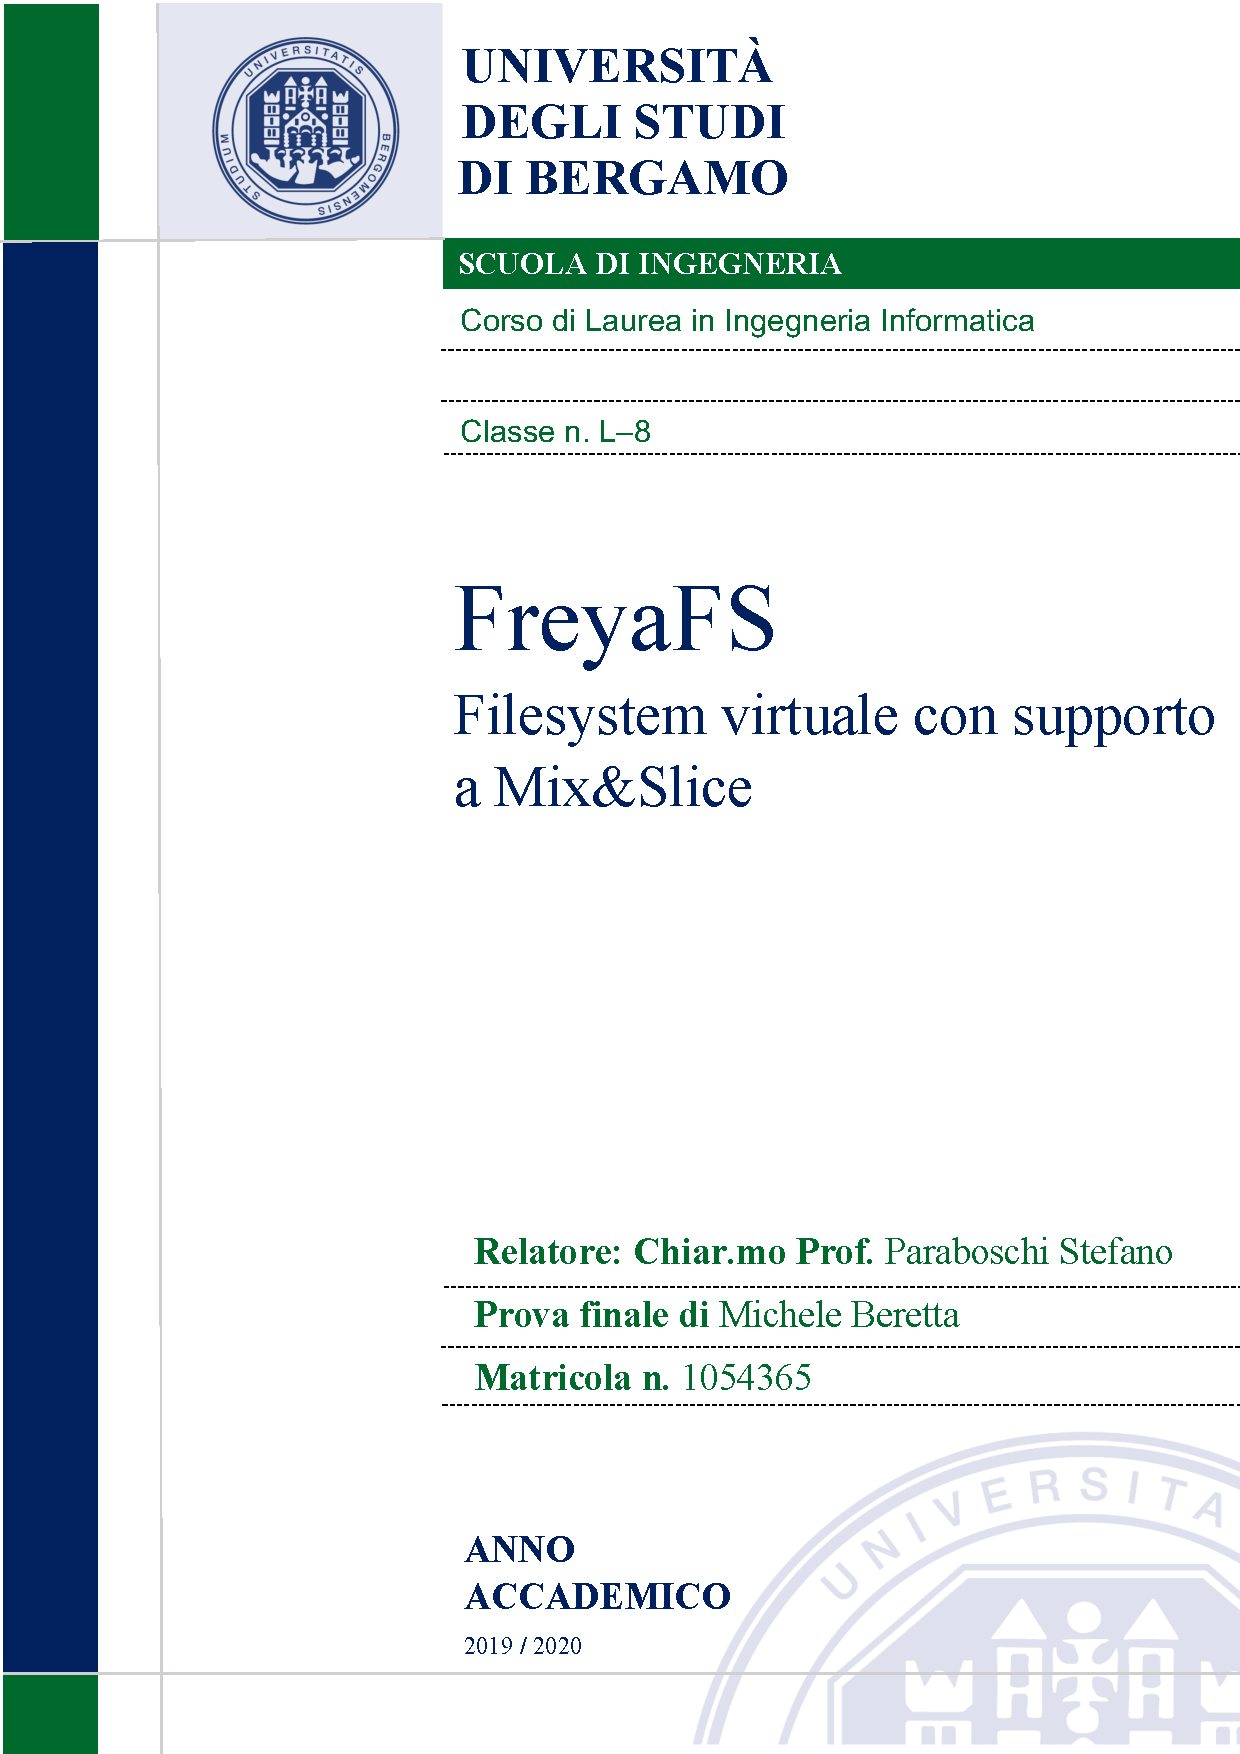
\includepdf[pages={1}]{frontespizio/frontespizio.pdf}

  % ----- EMPTY
  \clearpage
  \thispagestyle{plain}
  \pagenumbering{gobble}
  \mbox{}

  % ----- TITOLO
  \clearpage
  \maketitle
  
  % ----- EMPTY
  \clearpage
  \thispagestyle{plain}
  \pagenumbering{gobble}
  \mbox{}
  
  % ----- INDICE
  \clearpage
  \pagenumbering{Roman}
  \tableofcontents

  % ----- EMPTY
  \clearpage
  \thispagestyle{plain}
  \pagenumbering{gobble}
  \mbox{}

  \clearpage
  \pagenumbering{arabic}
  
  % ==================================================================
  % ====================== INTRODUZIONE ==============================
  % ==================================================================

  \chapter{Introduzione}
  \thispagestyle{fancy}
  
  % Scrivere perché hai scelto la tesi e quale è stato il risultato (come ci sei arrivato)

  Questa tesi tratta la realizzazione di un filesystem virtuale per GNU/Linux che supporti
  l'algoritmo di cifratura \textit{Mix\&Slice} in modo trasparente.

  Il filesystem realizzato si occuperà di gestire la creazione, la modifica e l'eliminazione di file e cartelle,
  sia da interfaccia grafica sia da riga di comando.

  \section{Contesto}

  Il motivo principale per il quale si rende necessaria la realizzazione di un filesystem che supporti
  la cifratura è la privacy dei dati.
  Spesso si hanno dei file (o, più in generale, delle informazioni) che vogliamo rendere accessibili solamente
  a poche persone per via della loro confidenzialità. Ciò è garantito dalla cifratura, che permette di proteggere
  le informazioni rendendole accessibili solamente a chi possiede una chiave.

  Si vuole però che l'utilizzo e l'accesso a questi dati sia il più semplice possibile, ovvero non sia
  in alcun modo diverso dall'accesso a file non criptati.
  Questa funzionalità viene realizzata dal filesystem virtuale, che cifra
  e decifra i file all'occorrenza, nascondendo le operazioni all'utente.

  \section{Il filesystem}

  \label{filesystem-descrizione}
  \subsection{Descrizione}

  Una delle funzioni principali di un sistema operativo è la gestione delle informazioni su
  memoria di massa, ovvero una qualsiasi unità periferica che non sia la memoria centrale.
  Il filesystem è il modulo del sistema operativo che si occupa di questo. Esso, in particolare,
  deve \cite{sistemioperativi}:

  \begin{itemize}
    \item fornire un meccanismo di identificazione univoco e permanente dei \textit{file}, affinché essi possano
          esistere ed essere accessibili per tempi lunghi;
    \item fornire dei \textit{metodi di accesso} che consentano di indirizzare, leggere e scrivere blocchi
          elementari di informazione contenuti nei file;
    \item mascherare le caratteristiche fisiche delle unità di memorizzazione;
    \item realizzare meccanismi di controllo di accesso sui file, sia per garantire riservatezza delle informazioni
          sia per evitare problemi di concorrenza;
    \item garantire la permanenza e la consistenza delle informazioni anche in caso di malfunzionamenti hardware o software.
  \end{itemize}

  Le principali strutture dati con cui un filesystem lavora sono i \textit{descrittori} dei file.
  I descrittori contengono varie proprietà del file, tra cui le principali sono il nome del file ed
  il suo indirizzo, ovvero la sua posizione in memoria di massa.
  Un insieme di descrittori è detto \textit{directory} (cartella). Dal momento che anche le cartelle devono
  essere memorizzate su disco permanentemente, esse vengono trattate dai sistemi Unix e Unix-Like
  al pari dei file: più precisamente, nel sistema Unix una cartella è un file che contiene la lista di nomi
  e indirizzi dei file contenuti al suo interno.

  \subsection{Operazioni sui file}

  Per poter accedere ad un file bisogna reperirne il descrittore dalla memoria di massa. Questa operazione però è
  computazionalmente pesante in termini di numero di accessi al disco. Di conseguenza, per risolvere
  questo problema, si introduce il concetto di \textit{apertura} del file: prima di una qualsiasi
  operazione sul file si ricerca il suo descrittore e se ne trasferisce il contenuto nella memoria centrale.
  Questo descrittore sarà poi adoperato per leggere e scrivere sul file in modo efficiente.
  
  Al termine dell'utilizzo di un file, segue l'operazione duale di \textit{chiusura}: l'immagine del descrittore
  contenuta in memoria centrale viene copiata su disco in modo da aggiornare le informazioni contenute nel file.

  Descriviamo l'apertura di un file come l'azione di ricerca e copia in memoria del
  descrittore di un file (ed eventualmente del suo contenuto) e la chiusura di un file come 
  l'atto del rilascio della memoria dedicata al descrittore, con conseguente trasferimento del contenuto su disco.

  \subsection{Filesystem virtuale}

  Un filesystem virtuale è un componente software che permette al kernel di un sistema operativo di accedere
  al filesystem tramite l'uso di funzioni standard e indipendenti dal filesystem reale (o dal dispositivo usato per la memorizzazione).

  L'accesso a file memorizzati su altri computer tramite la rete, o ancora l'accesso a file
  cifrati senza che l'utente si accorga della cifratura, sono esempi in cui il filesystem virtuale entra in gioco
  e semplifica l'interazione tra l'utente ed il computer.

  \subsection{FUSE - Filesystem in Userspace}

  FUSE è un'interfaccia software che consente la realizzazione di filesystem virtuali su kernel Linux \cite{libfusegithub}.
  Il progetto FUSE consta di due parti:
  \begin{enumerate}
    \item il modulo kernel per la comunicazione con il kernel Linux;
    \item la libreria utente \texttt{libfuse} che implementa la comunicazione tra il filesystem virtuale ed il modulo kernel;
  \end{enumerate}

  FUSE permette quindi all'utente di servirsi direttamente del meccanismo
  del filesystem virtuale su Linux e, in generale, sui sistemi Unix e Unix-like (tra cui FreeBSD e macOS)
  grazie ad un processo di porting e di riscrittura.

  \begin{figure}[h!]
    \centering
    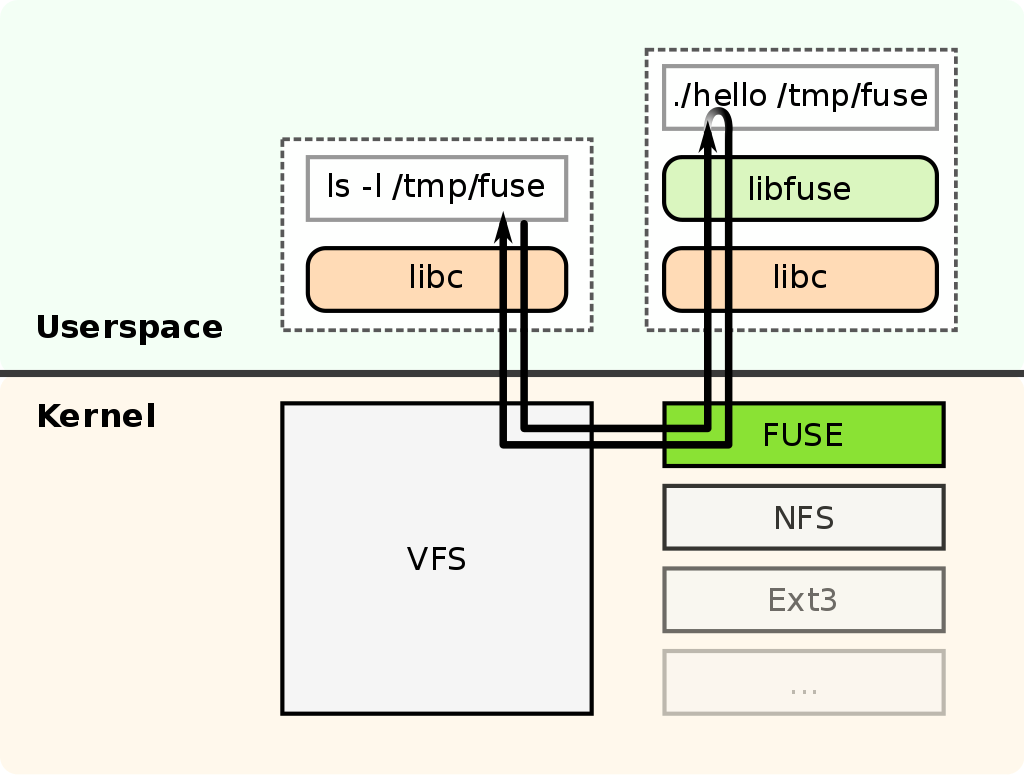
\includegraphics[width=0.6\linewidth]{images/fuse_structure.png}
    \caption{Funzionamento di FUSE}
    \label{fig:fuse-structure}
  \end{figure}

  Nella figura \ref{fig:fuse-structure} si può vedere un diagramma che rappresenta il funzionamento di FUSE
  con il kernel Linux.
  
  Ogni richiesta fatta dallo spazio utente (\texttt{ls -l /tmp/fuse}) viene intercettata
  dal modulo kernel VFS\footnotemark{} e viene reindirizzata al modulo kernel FUSE.
  La richiesta viene poi passata alla libreria utente \texttt{libfuse} che esegue
  un particolare programma configurato per gestire una specifica richiesta (\texttt{./hello}).
  La risposta del gestore viene quindi ceduta nuovamente a FUSE, per poi essere indirizzata infine
  al programma iniziale nello spazio utente.

  \footnotetext{Il \textit{Virtual Filesystem} \cite{linuxkernelvfs}, o \textit{Virtual Filesystem Switch},
  è un layer software del kernel Linux che fornisce l'interfacciamento tra il filesystem reale e lo spazio utente.}

  \section{La crittografia}

  \subsection{Descrizione ed utilità}
  La crittografia è una tecnica algoritmica che permette di rappresentare un messaggio in maniera offuscata,
  in modo da renderlo non comprensibile a persone non autorizzate a leggerne il contenuto.
  Il messaggio cifrato è detto \textit{crittogramma} ed i metodi usati sono detti \textit{tecniche di cifratura}.

  La crittografia si basa su un algoritmo ed una chiave di cifratura. L'algoritmo è spesso pubblico, mentre
  la chiave di cifratura è l'informazione che effettivamente garantisce la confidenzialità del messaggio:
  senza la chiave, non è possibile accedere alle informazioni cifrate.

  Le tecnologie informatiche ne fanno ampio utilizzo, ad esempio per
  garantire la privacy in un comunicazione tra due o più computer nella rete internet. 
  Essa può essere anche usata su file contenenti dati riservati, sensibili o semplicemente che non
  si desidera vengano resi disponibili pubblicamente.

  \subsection{Tipologie}

  Gli algoritmi di cifratura possono essere simmetrici o asimmetrici.

  Negli algoritmi \textit{simmetrici} si fa uso di un'unica chiave sia per cifrare sia per decifrare il messaggio.
  Pur essendo veloci, questi algoritmi hanno dei problemi di sicurezza che riguardano principalmente 
  proprio la presenza di un'unica chiave: questa dev'essere condivisa fra chiunque debba accedere alle
  informazioni cifrate, e se una terza persona ne viene in possesso può sia leggere il contenuto dei
  messaggi criptati sia modificarli.

  Negli algoritmi \textit{asimmetrici} invece si fa uso di due chiavi differenti, una per cifrare ed una per decifrare.
  Ad esempio, una chiave può essere resa pubblica ed essere usata per cifrare dei messaggi che solamente la persona
  in possesso dell'altra chiave potrà leggere.
  Lo svantaggio che comporta la crittografia asimmetrica è la lentezza.
  Infatti, se i dati da trasmettere sono tanti, è buona norma servirsi opportunamente di entrambi i metodi
  di cifratura: in primis si usa la crittografia asimmetrica per condividere una chiave, per poi utilizzare
  la crittografia simmetrica, meno computazionalmente pesante.

  \section{Filesystem criptati}

  Un filesystem criptato è un tipo particolare di filesystem in grado di trattare dei file cifrati.
  Affinché svolga le sue funzionalità è necessario fornirgli una chiave
  (o una coppia di chiavi) usata per la cifratura.
  I vantaggi di un filesystem criptato sono essenzialmente i seguenti:
  \begin{itemize}
    \item la \textit{privacy}, in quanto i file sono cifrati e non sono accessibili a persone che non conoscano la chiave di cifratura;
    \item la \textit{trasparenza}, in quanto le operazioni di cifratura e decifratura non sono visibili all'utilizzatore, che naviga tra i file come farebbe in un filesystem non cifrato;
  \end{itemize}

  Durante l'accesso alle informazioni, il filesystem cifra e decifra i file all'occorrenza,
  mantenendo su memoria di massa solamente i dati criptati.
  In questo modo, anche se si riuscisse ad avere accesso al supporto fisico di memorizzazione,
  non sarebbe possibile leggere il contenuto dei file.

  \section{Stato dell'arte}
  \subsection{EncFS}
  EncFS (\textit{Encrypted Filesystem}) \cite{encfsgithub} è una libreria open source
  rilasciata sotto licenza LGPL che implementa un filesystem virtuale con FUSE.
  EncFS cifra i file individualmente e traduce tutte le richieste per il filesystem virtuale nelle equivalenti chiamate
  al sistema operativo.

  In particolare, ha alcune funzionalità che lo distinguono da altri filesystem virtuali:
  \begin{itemize}
    \item ha una ``modalità inversa'', ossia fornisce una visione criptata di cartelle che non lo sono;
    \item è relativamente veloce su hard disk tradizionali;
    \item funziona anche con filesystem di rete;
  \end{itemize}

  \subsection{AONT - All-Or-Nothing Transform}
  Anche conosciuta come \textit{all-or-nothing-protocol}, AONT \cite{aontpaper} è una modalità di cifratura che permette
  di recuperare il contenuto del file solo se l'intero contenuto è accessibile.
  Quindi, se anche solo una parte del file criptato viene a mancare, l'intero file non è recuperabile.

  In particolare, una trasformazione $f$ è detta \textit{all-or-nothing transform} se:
  \begin{enumerate}
    % Reversibile o invertibile?
    \item è reversibile, ovvero è possibile ottenere il suo input se si ha a disposizione l'output;
    \item sia essa sia la sua inversa sono computabili in modo efficiente;
    \item non è computazionalmente possibile ricavare una qualsiasi parte dell'input se viene a mancare anche una sola parte dell'output;
  \end{enumerate}

  \subsection{Mix\&Slice}

  \textit{Mix\&Slice} \cite{mixslice} è un approccio che permette di imporre e gestire revoche di accesso a risorse criptate condivise.
  In modo simile a quanto si verifica con AONT, \textit{Mix\&Slice} rende impossibile ottenere
  la risorsa se non si ha accesso anche ad una parte della risorsa stessa criptata.
  Le tecniche di AONT non sono però applicabili in casi in cui gli utenti a cui è applicata la revoca
  sono a conoscenza delle chiavi di cifratura e potrebbero anche aver mantenuto una copia locale della risorsa criptata.

  L'approccio proposto da \textit{Mix\&Slice} richiede di partizionare la risorsa in tanti \textit{macro blocchi}, tutti della stessa dimensione,
  per poi applicare le due tecniche sulle quali esso si fonda:

  \begin{enumerate}
    \item \textit{Mixing}: il contenuto di ogni macro blocco è processato da diversi cicli di cifratura che ``mischiano''
          i bit del blocco. In questo modo, alla fine del processo, ogni bit di input ha un effetto su ogni bit di output.
    \item \textit{Slicing}: i macro blocchi sono quindi spezzati e raggruppati in \textit{frammenti}. Questi frammenti sono al
          centro dell'intero approccio, in quanto la mancanza di un qualsiasi frammento rende impossibile ricostruire la risorsa originale.
  \end{enumerate}

  \begin{figure}[h!]
    \centering
    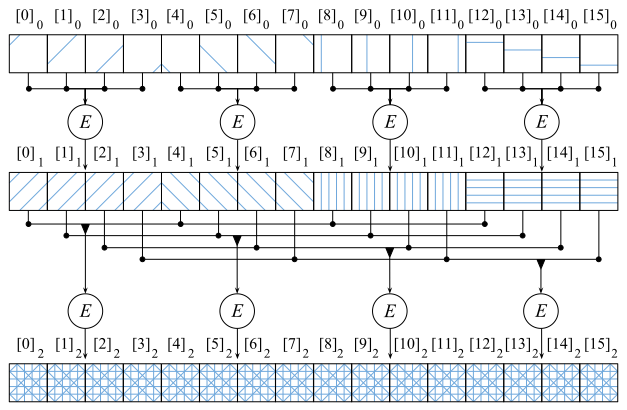
\includegraphics[width=0.7\linewidth]{images/mix_slice_example.png}
    \caption{Un esempio di \textit{Mix\&Slice}}
  \end{figure}

  % ==================================================================
  % ====================== SVILUPPO DEL PROGETTO =====================
  % ==================================================================

  \chapter{Sviluppo del progetto}
  \thispagestyle{fancy}

  \section{Ambiente e strumenti}

  Il filesystem virtuale è stato implementato con il linguaggio Python per il sistema operativo Ubuntu.
  Tra le librerie usate nel progetto sono presenti \texttt{fusepy} e \texttt{aesmix}.

  La libreria \texttt{fusepy} \cite{fusepygithub} è un modulo Python che offre dei bindings all'implementazione
  in C di FUSE per i sistemi Linux e macOS.

  L'utilità \texttt{aesmix} \cite{aesmixgithub} fornisce invece l'implementazione dell'algoritmo \textit{Mix\&Slice}
  per poter cifrare i file da utilizzare come test durante lo sviluppo.
  Questa mette a disposizione il wrapper Python \texttt{mixslice}, che permette di cifrare e decifrare un file utilizzando,
  appunto, \textit{Mix\&Slice}.

  Il wrapper Python accetta come input un file e scrive in output tre elementi:
  \begin{itemize}
    \item una cartella contenente i vari frammenti cifrati dati da \textit{Mix\&Slice};
    \item un file di metadati \texttt{.public}, che contiene la chiave pubblica;
    \item un file di metadati \texttt{.private}, che contiene la chiave privata.
  \end{itemize}

  I metodi principali di \texttt{aesmix} usati appartengono tutti alla classe \texttt{MixSlice} e sono i seguenti:
  \begin{itemize}
    \item \texttt{load\_from\_file}, che carica in memoria i file necessari alla decifratura;
    \item \texttt{save\_to\_files}, che salva i vari frammenti ed i file di metadati su disco;
    \item \texttt{encrypt}, per cifrare un file;
    \item \texttt{decrypt}, per decifrare un file.
  \end{itemize}

  \section{Logica e funzionamento}

  \subsection{Mountpoint, cartella di dati e cartella di metadati}

  Il filesystem virtuale necessita di tre cartelle per poter essere montato ed utilizzato:

  \begin{enumerate}
    \item una che indica il mountpoint, ovvero il punto dove verrà montato il \mbox{filesystem} virtuale;
    \item una contenente i vari dati cifrati, eventualmente organizzati in sottocartelle;
    \item una che fornisce tutti i file di metadati (\texttt{.public}, \texttt{.private} e \texttt{.finfo}).
  \end{enumerate}

  Le cartelle dei file cifrati e dei file di metadati sono diverse tra loro per poter consentire
  una generalità nell'utilizzo del filesystem.
  È necessario che la struttura di entrambe sia la stessa per garantire univocità nell'associazione tra file
  cifrato e file di metadati corrispondente, poiché possono esistere file con nomi uguali in diversi punti
  del filesystem.

  Ad esempio, se un file cifrato ha il percorso \texttt{dir/immagine.png}, allora i suoi file di metadati
  dovranno essere \texttt{dir/immagine.png.public},
  \texttt{dir/immagine.png.private} e \texttt{dir/immagine.png.finfo}.
  
  Dal momento che l'utilità \textit{aesmix} dà in output una cartella che contiene i frammenti, per
  distinguere tra cartella e file cifrato il filesystem fa riferimento all'esistenza o meno
  dei file di metadati: se per un dato percorso sono presenti i relativi file di metadati
  allora esso viene trattato come se fosse un file cifrato, altrimenti la gestione viene lasciata
  al sistema operativo.

  \subsection{Gestione di file criptati}
  \label{section-file-criptati}

  Il filesystem deve mostrare le cartelle contenenti i frammenti cifrati come dei file.
  Per fare in modo che ciò avvenga è necessario cambiare le informazioni che si trovano nel
  descrittore del file visto dal sistema.
  Dal momento che le cartelle sono dei file, anche per esse viene recuperato il descrittore corrispondente
  in modo del tutto analogo a come avviene per i file (vedi sezione \ref{filesystem-descrizione}).
  
  Alla richiesta del descrittore da parte del sistema, vengono quindi modificate le seguenti proprietà \cite{linuxmanstat}:
  \begin{itemize}
    \item \texttt{st\_mode}: contiene i permessi ed il tipo di file. Per far apparire le cartelle cifrate come
          dei file si impone il flag \texttt{S\_IFREG}, che identifica un file, e si rimuove il flag
          \texttt{S\_IFDIR}, che identifica una cartella. Gli altri permessi rimangono invariati.
    \item \texttt{st\_nlink}: il numero di hard link del file. Questo è pari a $2$ per una cartella, quindi si
          impone a $1$ per far apparire le cartelle cifrate come file.
    \item \texttt{st\_size}: la dimensione in Byte del file.
  \end{itemize}

  In particolare, per trovare la dimensione reale del file, è stato necessario decifrare il file stesso
  poiché il sistema operativo utilizza il campo \texttt{st\_size} per sapere quanti Byte leggere da disco\footnotemark.
  Infatti, in un primo momento era stata mantenuta la dimensione totale della cartella (ovvero la somma delle dimensioni
  dei frammenti in essa contenuti) e questo poteva causare dei problemi alla lettura del file, soprattutto da interfaccia grafica.
  All'apertura del file, il sistema poteva leggere meno Byte di quanti ne contenesse il file, considerando quindi il file corrotto, oppure
  leggere più Byte del dovuto, andando in crash e richiedendo una chiusura forzata dell'applicazione.
  \footnotetext{Questo non è un comportamento comune a tutto il sistema, infatti è adottato dall'interfaccia
  grafica ma non da linea di comando. Da terminale, anche con un valore di \texttt{st\_size} sbagliato, è
  possibile leggere il contenuto di un file con \texttt{cat} e scriverlo tramite la combinazione di
  \texttt{echo} e \texttt{>}.}

  Decifrare un file ogni volta che viene fatta una richiesta del descrittore può però causare rallentamenti.
  Per questo motivo è stato introdotto un nuovo tipo di file di metadati, con estensione \texttt{.finfo}, che contiene 
  informazioni sulla dimensione dei file nel filsystem virtuale. Questa dimensione viene aggiornata
  ad ogni scrittura e troncatura sul file, solamente se è effettivamente cambiata.
  In questo modo, seppur con un overhead iniziale dovuto alla scrittura su file, il filesystem risulta
  decisamente più reattivo nel suo utilizzo normale.

  Quanto descritto in questa sezione può essere fatto solamente se è possibile aprire e decifrare il file
  e se esistono dei file di metadati associati ad esso.
  Le cartelle che non contengono i frammenti cifrati vengono quindi trattate direttamente dal sistema,
  che le gestisce senza modifiche da parte del filesystem virtuale.

  \subsection{Lettura, scrittura e creazione di file}

  Per poter leggere e scrivere un file è necessario aprirlo, ovvero decifrarlo e trasferire il suo contenuto in memoria.

  La \textit{lettura} avviene a blocchi sul contenuto in memoria, tramite un offset e un numero totale di Byte da leggere.
  La \textit{scrittura}, invece, avviene tramite un buffer con i dati da salvare ed un offset che indica il Byte da cui
  iniziare a scrivere. È anche possibile \textit{troncare} un file, ovvero limitarne la lunghezza ad un certo valore, eliminando
  qualsiasi informazione in eccesso. All'apertura viene impostato anche il nuovo valore da dare a \texttt{st\_atime},
  che indica l'istante temporale dell'ultimo accesso al file \cite{linuxmanstat}.

  La \textit{scrittura} ha la particolarità di non essere effettuata su disco direttamente, ma viene effettuata
  sul contenuto del file in memoria. Il file viene cifrato su disco in un momento successivo, al
  flush del file. Per motivi di efficienza, il flush viene fatto solamente se sono state eseguite
  delle modifiche al contenuto del file, ovvero se è stata fatta almeno una scrittura.
  In questo modo, se un file non è stato modificato da quando è stato aperto non si effettuano cifrature non
  necessarie, rendendo più veloci le operazioni di sola lettura.
  La scrittura inoltre si occupa di cambiare il valore di \texttt{st\_mtime}, che indica
  l'istante (Unix timestamp) di ultima modifica \cite{linuxmanstat} al contenuto del file.

  La \textit{creazione} di un file su disco corrisponde alla creazione in memoria di un'area con il dovuto contenuto,
  anche vuoto\footnote{Se si tenta di creare un file già esistente o già aperto, il contenuto di questo dev'essere mantenuto
  e non dev'essere sovrascritto.}, ed al flush forzato del file. Inoltre, la creazione di un file abilita alla possibilità
  di copiare e duplicare i file, in quanto la copia è sostanzialmente una creazione seguita da una o più scritture.

  \subsection{Rinomina ed eliminazione di file}

  La \textit{rinomina} di un file cifrato comporta anche la rinomina dei file di metadati associati.
  Se fatta da interfaccia grafica, l'operazione non permette la rinomina in un file già esistente,
  mentre da linea di comando la rinomina è indistinguibile dallo spostamento di un file.
  L'implementazione di una corretta rinomina abilita quindi sia la possibilità di spostare i file
  sia la possibilità di sovrascrivere i file nel filesystem virtuale.
  
  L'\textit{eliminazione} definitiva di un file comporta anche l'eliminazione dei file di metadati.
  Lo spostamento nel cestino, invece, è a tutti gli effetti uno spostamento, quindi supportato con la rinomina.
  Se sul volume virtuale creato da FUSE non esiste una cartella adibita a cestino, questa verrà creata.
  Anche i file nel cestino saranno cifrati.

  Né l'eliminazione né la rinomina necessitano di apertura e chiusura dei file, quindi risultano particolarmente
  performanti per l'assenza di cifrature e decifrature.
  Entrambe le operazioni, però, necessitano di modificare le informazioni mantenute in memoria
  riguardanti le varie caratteristiche dei file, per evitare di fare riferimento a dati non più validi
  (vedi la gestione di \texttt{st\_size} alla sezione \ref{section-file-criptati} e l'implementazione
  di \texttt{EncFilesManager} a \ref{enc-files-manager}).
  Può anche capitare che un file venga rinominato mentre è aperto.

  \subsection{Aperture multiple dello stesso file}
  \label{aperture-multiple-file}

  Un file può essere aperto contemporaneamente da più applicazioni. Alla chiusura di una
  di queste, il filesystem impedisce la chiusura di un file se è ancora in uso da
  altri programmi, per evitare comportamenti indesiderati o corruzione dei dati.

  Questo si traduce operativamente nel mantenere un contatore per ogni file aperto in memoria,
  che è incrementato ad ogni apertura e decrementato ad ogni chiusura del file in questione.
  Il file viene infine chiuso, rilasciando le aree di memoria dedicate, quando questo
  contatore arriva al valore 0. Resta possibile effettuare più volte il flush di un file
  per aggiornarne il contenuto su disco.

  Le applicazioni si occupano da sé di aggiornare il contenuto del file se
  questo è cambiato su disco, oppure propongono all'utente di ricaricarlo. Questo avviene
  grazie all'aggiornamento di \texttt{st\_mtime} durante le operazioni di scrittura.

  \subsection{Gestione di cartelle}

  Per mantenere la stessa identica struttura tra la cartella con i file cifrati e la cartella
  con i file di metadati, il filesystem virtuale deve occuparsi di replicare 
  tutte le operazioni sulle cartelle (creazione, modifica ed eliminazione) tra le due posizioni su disco.

  La gestione non presenta particolari difficoltà, fatta eccezione per l'operazione
  di rinomina, in quanto essa è effettuata dal sistema operativo tramite la stessa primitiva usata
  per i file, \texttt{rename},
  a differenza di altre operazioni: ad esempio, per rimuovere un file si usa il metodo \texttt{unlink},
  mentre per rimuovere una cartella si usa il metodo \texttt{rmdir}.
  Nel caso della rinomina è quindi necessario differenziare tra file cifrato e cartella tramite la proprietà
  \texttt{st\_mode} del descrittore opportunamente modificato, come spiegato nella sezione \ref{section-file-criptati}.

  \subsection{Multithreading}

  La libreria \texttt{libfuse} di Linux permette di montare i filesystem virtuali in due modalità:
  \begin{enumerate}
    \item \textit{single-thread}, in cui l'intero filesystem viene eseguito su un solo thread all'interno di un processo;
    \item \textit{multi-thread}, in cui le varie operazioni (scrittura, lettura, etc.) sono assegnate ogni volta a thread diversi.
  \end{enumerate}

  La modalità single-thread è meno performante dal punto di vista prestazionale
  ma è più semplice e adatta allo sviluppo poiché non richiede nessun controllo di concorrenza.

  La modalità multi-thread offre invece performance migliori in quanto consente di parallelizzare le operazioni
  sui file quando possibile, come per esempio nel caso di una lettura di una grande quantità di dati.
  Nello specifico, la libreria \texttt{libfuse} protegge le sezioni critiche del codice da accessi concorrenti tramite
  semafori implementati secondo lo standard POSIX tramite la libreria \texttt{pthread.h}.

  \textit{FreyaFS} mantiene questi due paradigmi, operando di default su un singolo \mbox{thread}.
  Sebbene \texttt{libfuse} si occupi già a basso livello della protezione delle sezioni critiche,
  resta comunque necessario proteggere l'accesso alle zone di memoria condivise,
  rappresentate principalmente dal contenuto dei file aperti ed i contatori delle applicazioni
  che hanno aperto un dato file.
  
  Il filesystem gestisce in modo diverso le azioni di scrittura e di lettura del contenuto dei file aperti.
  Più letture possono avvenire in parallelo al fine di aumentare le prestazioni, mentre le scritture non devono
  interferire le une con le altre e devono avere l'accesso esclusivo alla risorsa.
  Questo comportamento è realizzato tramite l'utilizzo di \textit{read lock} e \textit{write lock}.
  Il filesystem virtuale mantiene per ogni file aperto un contatore di quanti thread stanno leggendo la risorsa:
  questo viene incrementato ogni volta che ad un thread inizia l'operazione di lettura e decrementato quando termina.
  Quando un thread richiede l'accesso in scrittura al file viene messo in attesa se sono presenti dei lettori
  e viene notificato quando non ce ne sono più. Se invece la risorsa è libera viene garantito l'accesso in modo
  esclusivo tramite un semaforo.

  \section{Implementazione}

  Il progetto è organizzato in cinque file principali:

  \begin{itemize}
    \item \texttt{main.py}, che si occupa della gestione degli argomenti da linea di comando e del montaggio del filesystem;
    \item \texttt{freyafs.py}, che gestisce il funzionamento del filesystem in generale e comunica con il sistema operativo;
    \item \texttt{encfilesmanager.py}, che implementa le varie operazioni di input/output sui file;
    \item \texttt{encfilesinfo.py}, che gestisce i file di metadati \texttt{.finfo};
    \item \texttt{filebytecontent.py}, che si occupa della gestione della concorrenza sul contenuto dei file in memoria.
  \end{itemize}

  Nella figura \ref{struttura-statica} si vede la struttura statica del codice, in particolare come i
  moduli sono in relazione tra loro. Una freccia da un modulo A ad un modulo B indica che B usa il modulo A.
  Nei moduli ``esterni'' sono rappresentati \texttt{aesmix}, che realizza l'implementazione di \textit{Mix\&Slice},
  e \texttt{fusepy}, che fornisce l'implementazione di FUSE per il linguaggio Python.
  I moduli ``interni'' sono quelli che si occupano di gestire i file cifrati e che compongono a tutti
  gli effetti la logica del filesystem virtuale.
  Infine, \texttt{main} gestisce solamente l'interfacciamento con l'utente da riga di comando
  e fa uso di \texttt{fusepy} per montare il filesystem.

  \begin{figure}
    \centering
    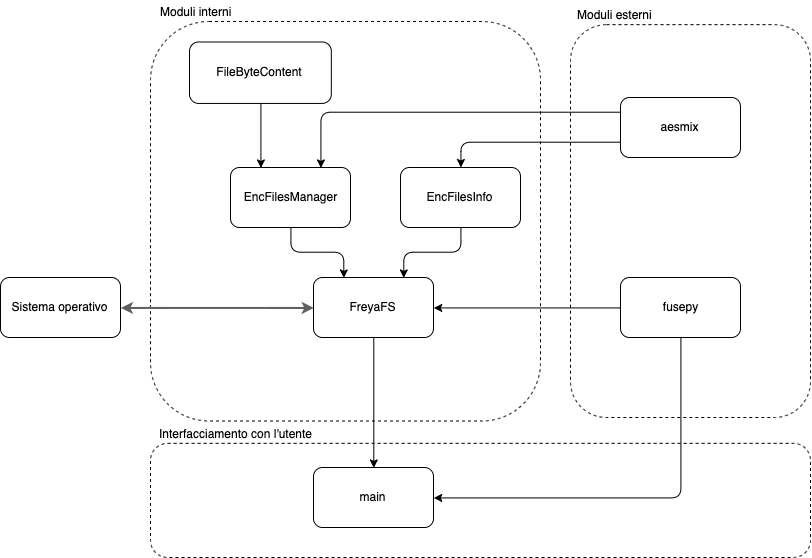
\includegraphics[width=0.8\linewidth]{images/code-diagram.png}
    \caption{Struttura del codice}
    \label{struttura-statica}
  \end{figure}

  \subsection{Interfacciamento con l'utente}

  L'interfacciamento con l'utente è gestito dal modulo \texttt{main.py}, che si occupa di organizzare
  gli argomenti passati da riga di comando e di montare il filesystem.
  I parametri che è possibile impostare sono presenti nella tabella \ref{table-main}.

  \begin{table}[h!]
    \centering
    \begin{tabular}{|p{4.5cm}|p{9.5cm}|} 
      \hline
      Parametro & Utilizzo \\ [0.5ex] 
      \hline\hline
      \texttt{MOUNT} & Il mountpoint, ovvero il percorso dove verrà montato il filesystem \\ 
      \hline
      \texttt{-{}-data DATA} & Il percorso della cartella contenente i file cifrati \\
      \hline
      \texttt{-{}-metadata METADATA} & Il percorso della cartella dei file di metadati \\
      \hline
      \texttt{-{}-multithread} & Flag che indica se montare il filesystem in modalità multi-thread (di default a \texttt{False}) \\
      \hline
    \end{tabular}
    \caption{Parametri di \texttt{main.py}}
    \label{table-main}
  \end{table}
  
  
  \subsection{FreyaFS}

  Il modulo \texttt{freyafs} implementa i metodi di FUSE per la gestione del filesystem virtuale.
  In particolare, la parte più importante del modulo è la classe
  \texttt{FreyaFS}, che estende la classe \texttt{Operations} di FUSE e ne ridefinisce alcuni metodi, facendone
  l'overloading. Molti dei metodi della classe richiamano semplicemente il sistema operativo, in quanto
  non necessitano del supporto alla cifratura (come ad esempio il test di accesso ad un file).
  Altri metodi, invece, sono ridefiniti per supportare la cifratura e decifratura dei file, realizzata
  dal modulo \texttt{encfilesmanager}.

  Di seguito un estratto del metodo \texttt{getattr}, usato per ricavare informazioni del descrittore
  di file e cartelle. Il codice qui presente riguarda la modifica delle informazioni
  del descrittore delle cartelle contenenti i frammenti cifrati.

  \begin{lstlisting}[language=Python]
  if full_path not in self.enc_info:
    public_metadata, _, finfo = self._metadata_names(path)
    self.enc_info[full_path] = EncFilesInfo(full_path, public_metadata, finfo)

  return {
      'st_mode': stat.S_IFREG | (st.st_mode & ~stat.S_IFDIR),
      'st_nlink': 1,
      'st_atime': st.st_atime,
      'st_ctime': st.st_ctime,
      'st_gid': st.st_gid,
      'st_mtime': st.st_mtime,
      'st_size': self.enc_info[full_path].size,
      'st_uid': st.st_uid
  }
  \end{lstlisting}

  Questo frammento di codice ha due compiti principali: il calcolo della dimensione del file cifrato e il cambio di
  flag per far apparire la cartella coi frammenti come un unico file.
  
  Il calcolo della dimensione è fatto dall'istanziamento della classe
  \texttt{EncFilesInfo}, solo se non già stato effettuato in precedenza (al fine di migliorare le prestazioni
  evitando decifrature sovrabbondanti, righe dalla 1 alla 3).
  La proprietà \texttt{self.enc\_info} è un dizionario che contiene le varie istanze di \texttt{EncFilesInfo}
  per ogni file cifrato trovato nel sistema.

  Il cambio di flag viene effettuato in modo da mantenere gli stessi permessi, come si evince dall'espressione
  alla riga 6, dove \texttt{st.st\_mode} sono i permessi originali della cartella con i frammenti.
  Il flag \texttt{stat.S\_IFREG} è alzato tramite un'operazione di \texttt{OR} bit a bit, mentre per abbassare il
  flag \texttt{stat.S\_IFDIR} è necessario fare un \texttt{AND} bit a bit
  con la negazione bit a bit di \texttt{stat.S\_IFDIR}, ovvero \texttt{st.st\_mode \& \textasciitilde stat.S\_IFDIR}.

  Segue un estratto del metodo \texttt{unlink}, che consente la rimozione dei file.
  \begin{lstlisting}[language=Python]
  full_path = self._full_path(path)
  public_metadata, private_metadata, finfo = self._metadata_names(path)

  os.unlink(public_metadata)
  os.unlink(private_metadata)
  if os.path.isfile(finfo):
      os.unlink(finfo)

  if full_path in self.enc_info:
      del self.enc_info[full_path]

  shutil.rmtree(full_path)
  \end{lstlisting}

  Nel codice vengono solamente chiamate le primitive del sistema operativo, senza aprire o chiudere
  nessun file. Vengono anche eliminati i file di metadati e le zone di memoria dedicate
  alle informazioni dei file (riga 10).
  È necessario controllare l'esistenza del file \texttt{.finfo} (riga 6) perché,
  a differenza di \texttt{.public} e \texttt{.private}, può non esistere
  in quanto viene creato alla prima chiamata di \texttt{getattr} per il file in questione.

  La rinomina di un file, gestita dal metodo \texttt{rename}, risulta invece più complessa, in quanto
  è la stessa operazione usata per lo spostamento sia di file sia di cartelle.
  Inoltre, siccome i file cifrati sono cartelle, se si vuole rinominare un file con un nome di un altro file già
  esistente\footnote{Questo comportamento è impedito da interfaccia grafica, ma consentito da linea di comando con il comando \texttt{mv}.}
  bisogna prima eliminare quest'ultimo (righe 6-7), per evitare che il sistema lo riconosca come cartella e
  tenti di spostare il primo ``dentro'' il secondo.
  Infine, sono anche rinominati i percorsi presenti in memoria relativi al file ed ai suoi metadati (righe 19-25).

  Per le cartelle ``normali'', ovvero non contenenti frammenti cifrati,
  la rinomina è lasciata al sistema operativo e replicata sia
  nel percorso dei dati cifrati sia nel percorso dei metadati (caso \texttt{else}).
  \begin{lstlisting}[language=Python]
  full_old_path = self._full_path(old)
  full_new_path = self._full_path(new)

  if self._is_file(old):
      # Rinomino un file
      if self._is_file(new):
          self.unlink(new)

      old_public_metadata, old_private_metadata, old_finfo = self._metadata_names(old)
      new_public_metadata, new_private_metadata, new_finfo = self._metadata_names(new)

      os.rename(old_public_metadata, new_public_metadata)
      os.rename(old_private_metadata, new_private_metadata)
      if os.path.isfile(old_finfo):
          os.rename(old_finfo, new_finfo)

      os.rename(full_old_path, full_new_path)

      if full_old_path in self.enc_files:
          self.enc_files.rename(full_old_path, full_new_path)
      
      if full_old_path in self.enc_info:
          self.enc_info[full_old_path].rename(full_new_path, new_public_metadata, new_finfo)
          self.enc_info[full_new_path] = self.enc_info[full_old_path]
          del self.enc_info[full_old_path]
  else:
      # Rinomino una cartella
      old_metadata_path = self._metadata_full_path(old)
      new_metadata_path = self._metadata_full_path(new)            
      os.rename(old_metadata_path, new_metadata_path)
      os.rename(full_old_path, full_new_path)
  \end{lstlisting}

  Tutti i metodi che agiscono su input ed output di file, invece,
  richiamano i dovuti metodi della classe \texttt{EncFilesManager} e, se necessario, aggiornare
  la lunghezza corrente gestita da \texttt{EncFilesInfo}. A scopo esemplificativo, di seguito
  viene riportato il metodo \texttt{write}.

  \begin{lstlisting}[language=Python]
  def write(self, path, buf, offset, fh):
      full_path = self._full_path(path)
      if full_path in self.enc_files:
          bytes_written = self.enc_files.write_bytes(full_path, buf, offset)
          self._update_enc_file_size(full_path)
          return bytes_written

      os.lseek(fh, offset, os.SEEK_SET)
      return os.write(fh, buf)
  \end{lstlisting}
  
  In questi due estratti, \texttt{self.enc\_files} è un'istanza della classe \texttt{EncFilesManager} che contiene
  tutti i contenuti dei file attualmente aperti, in modo da poterli leggere e scrivere.

  I metodi di \texttt{open}, \texttt{create}, \texttt{truncate}, \texttt{read}, \texttt{flush} e \texttt{release}
  hanno tutti una struttura similare. Se un file non risulta aperto tra quelli cifrati, allora il file viene
  gestito dal sistema operativo come farebbe di consueto.

  In conclusione, la tabella \ref{table-freyafs} riassume alcuni metodi usati da \textit{FreyaFS} che è stato
  necessario modificare rispetto al caso considerato ``base'', ovvero il caso in cui per ogni metodo vengono
  semplicemente richiamate le primitive del sistema operativo corrispondenti.

  \begin{table}[h!]
    \centering
    \begin{tabular}{|p{3cm}|p{11cm}|} 
      \hline
      Metodo & Utilizzo \\ [0.5ex] 
      \hline\hline
      \texttt{getattr} & Ottiene le informazioni di un file cifrato o cartella \\ 
      \hline
      \texttt{readdir} & Fornisce il contenuto di una data cartella, includendo \texttt{.} e \texttt{..} ed ignorando file di metadati \\
      \hline
      \texttt{mkdir} & Crea una cartella, sia nel percorso dei dati cifrati sia nel percorso dei metadati \\
      \hline
      \texttt{rmdir} & Rimuove una cartella, sia nel percorso dei dati cifrati sia nel percorso dei metadati \\
      \hline
      \texttt{unlink} & Rimuove un file cifrato, eliminando anche i corrispondenti file di metadati \\
      \hline
      \texttt{rename} & Rinomina un file cifrato (ed i corrispondenti file di metadati) o una cartella \\
      \hline
      \texttt{utimens} & Aggiorna gli istanti di ultimo aggiornamento e di ultima modifica per file cifrati e per cartelle \\
      \hline
      \texttt{open} & Apre un file cifrato \\
      \hline
      \texttt{create} & Crea un file cifrato \\
      \hline
      \texttt{read} & Legge un certo numero di Byte da un file cifrato aperto \\
      \hline
      \texttt{write} & Scrive un certo numero di Byte in un file cifrato aperto \\
      \hline
      \texttt{truncate} & Tronca il contenuto di un file cifrato aperto ad una data lunghezza \\
      \hline
      \texttt{flush} & Forza le scritture fatte su in file cifrato dalla memoria al disco \\
      \hline
      \texttt{release} & Rilascia un file cifrato aperto \\
      \hline
    \end{tabular}
    \caption{Metodi di \textit{FreyaFS}}
    \label{table-freyafs}
  \end{table}

  \subsection{EncFilesManager}
  \label{enc-files-manager}

  Questo modulo definisce la classe omonima per l'input ed output sui file cifrati.
  In particolare, la classe viene istanziata una sola volta e contiene le informazioni di tutti
  i file (cifrati con \textit{Mix\&Slice}) al momento aperti, identificabili tramite il loro
  percorso nel filesystem reale.
  Si serve di un contatore per ogni file aperto che indica quante applicazioni lo stanno
  usando al momento: in questo modo si evita di chiudere ``accidentalmente'' il file se solamente
  alcune di queste applicazioni lo rilasciano mentre altre devono mantenerlo ancora aperto.

  I metodi definiti sono i seguenti:

  \begin{itemize}
    \item \texttt{open}: apre un file, decifrandone il contenuto e mantenendolo in memoria;
    \item \texttt{create}: crea un file vuoto, ovvero riserva dello spazio vuoto in memoria per il contenuto del file
      (solo se non già aperto) e ne impone il flush;
    \item \texttt{read\_bytes}: legge un certo numero di Byte da un file aperto;
    \item \texttt{write\_bytes}: sovrascrive una parte del contenuto di un file aperto con dei dati contenuti in buffer;
    \item \texttt{truncate\_bytes}: tronca il contenuto di un file aperto ad una certa lunghezza;
    \item \texttt{flush}: scrive il contenuto di un file aperto su disco, cifrandolo;
    \item \texttt{release}: rilascia le aree di memoria dedicate ad un file, chiudendolo;
    \item \texttt{cur\_size}: ottiene la lunghezza attuale del contenuto di un file aperto;
    \item \texttt{rename}: rinomina i vari percorsi riferiti ad un file aperto.
  \end{itemize}

  È fondamentale avere un metodo \texttt{rename} perché un file può essere rinominato anche se aperto:
  in questo caso, per evitare di fare riferimento a file non più esistenti e causare un comportamento
  errato del filesystem, bisogna aggiornare tutti i percorsi relativi al file in questione.

  La classe \texttt{EncFilesManager} tiene anche traccia dello stato di modifiche di un file tramite dei flag booleani.
  In questo modo, se viene richiesto un \texttt{flush} ma non sono presenti modifiche al file, è possibile
  evitare l'operazione di cifratura per migliorare le prestazioni del filesystem ed evitare tempi morti essenzialmente inutili.

  Infine, la classe gestisce anche la mutua esclusione per la modalità multi-thread del filesystem virtuale,
  tramite un semaforo di tipo \texttt{Lock} del modulo \texttt{threading} di Python (vedere la sezione \ref{section-lib-threading}).
  Questo semaforo garantisce l'accesso esclusivo alle strutture che contengono il contenuto dei
  file aperti ed i contatori dei file aperti.

  Il codice qui riportato è l'implementazione del metodo \texttt{open}:
  \begin{lstlisting}[language=Python]
  def open(self, path, public_metafile_path, private_metafile_path, mtime):
    with LOCK:
        if path in self.open_files:
            self.open_counters[path] += 1
            return

        self.public_metafiles[path] = public_metafile_path
        self.private_metafiles[path] = private_metafile_path

        self.open_files[path] = FileByteContent(self._decrypt(path))
        self.open_counters[path] = 1
    
    self.touched_files[path] = False
    self.atimes[path] = int(time())
    self.mtimes[path] = mtime
  \end{lstlisting}

  Il metodo si occupa anche di aggiornare il timestamp di ultimo accesso al file,
  tramite \texttt{self.atimes}, ed il timestamp di ultima modifica al file, tramite \texttt{self.mtimes}.
  Tra i due, solamente il secondo viene aggiornato durante le scritture sul contenuto del file
  ed entrambi sono sempre scritti su disco al flush del file, anche in caso di assenza di modifiche.

  \subsection{EncFilesInfo}

  Il modulo \texttt{encfilesinfo} definisce la classe \texttt{EncFilesInfo} che si occupa di gestire varie informazioni dei
  file cifrati che non sono contenute nei file di metadati \texttt{.private} e \texttt{.public}.
  Il suo compito principale è interfacciare \texttt{freyafs} con i file \texttt{.finfo}, che contengono le varie
  informazioni serializzate come JSON.
  La classe, a differenza di \texttt{EncFilesManager}, non è a conoscenza di tutti i file trovati dal filesystem
  virtuale, ma gestisce solamente le informazioni di un singolo file specificato all'inizializzazione.

  Al momento il modulo supporta solamente la gestione della lunghezza in Byte del contenuto del file cifrato,
  che si può ottenere ed impostare tramite la proprietà \texttt{size}.
  
  All'istanziamento della classe, viene calcolata la dimensione del file cifrato desiderato e
  viene memorizzata nella proprietà \texttt{size} e anche nel file \texttt{.finfo} (che, se non presente, viene creato).
  Quando si vuole modificare questa proprietà, viene anche aggiornato il valore contenuto nel file
  di metadati solamente se il valore è diverso da quello precedente. In questo modo si evita
  di aprire un file, effettuare il parsing del JSON in esso contenuto, aggiornare la proprietà per poi
  serializzare nuovamente il JSON prodotto nel caso in cui queste operazioni non siano
  strettamente necessarie.
  \begin{lstlisting}[language=Python]
  @property
  def size(self):
      if self._size is None:
          self._size = size_decrypt(self._path, self._public_metadata)
          self._update_finfo()
      return self._size

  @size.setter
  def size(self, value):
      if self._size == value:
          return
      self._size = value
      self._update_finfo()
  \end{lstlisting}

  La classe mette anche a disposizione un metodo \texttt{rename}, usato per rinominare i
  percorsi del file di cui mantiene le informazioni.

  \subsection{FileByteContent}
  \label{section-filebytecontent}

  Questo modulo si occupa unicamente di effettuare letture e scritture sul contenuto
  in memoria di un file aperto in modo mutualmente esclusivo.
  Per garantire ciò, la classe \texttt{FileByteContent} ha le seguenti proprietà:
  \begin{itemize}
    \item \texttt{\_text}, che rappresenta il contenuto del file come stringa di Byte;
    \item \texttt{\_readers}, che indica il numero di lettori presenti in un dato momento;
    \item \texttt{\_cond}, di tipo \texttt{threading.Condition} che viene usata come semaforo.
  \end{itemize}

  La classe \texttt{FileByteContent} consente di avere un semaforo per ogni file aperto.
  In questo modo, sono possibili letture e scritture parallele su file diversi, ma non sullo stesso file.

  A scopo esemplificativo, di seguito alcuni metodi della classe.
  \begin{lstlisting}[language=Python]
  def read_bytes(self, offset, length):
      self._r_acquire()
      text = self._text[offset:offset + length]
      self._r_release()
      return text

  def write_bytes(self, buf, offset):
      self._w_acquire()
      bytes_written = len(buf)
      new_text = self._text[:offset] + buf + self._text[offset+bytes_written:]
      self._text = new_text
      self._w_release()
      return bytes_written

  def truncate(self, length):
      self._w_acquire()
      self._text = self._text[:length]
      self._w_release()
  \end{lstlisting}

  In questo estratto di codice \texttt{\_r\_acquire()} e \texttt{\_r\_release()} si occupano rispettivamente di acquisire e rilasciare
  il lock in lettura, condivisibile tra più thread, mentre \texttt{\_w\_acquire()} e \texttt{\_w\_release()}
  sono l'equivalente per il lock in scrittura, che garantisce l'accesso esclusivo al contenuto del file.

  L'acquisizione di un lock per la lettura incrementa la variabile \texttt{\_readers}, che viene 
  decrementata con il rilascio. Quando si raggiunge lo $0$, si notificano eventuali thread in attesa di scrittura.

  Alla richiesta di un lock in scrittura, il thread rimane in attesa fintantoché sono presenti
  dei lettori, ovvero se \texttt{\_readers} è positiva. Quando i lettori liberano la risorsa, viene acquisito
  il lock e viene rilasciato al termine dell'operazione.

  I metodi per l'acquisizione ed il rilascio dei lock di lettura e scrittura sono implementati
  come segue.
  Per dettagli più specifici sulla proprietà \texttt{\_cond} fare riferimento alla
  sezione \ref{section-lib-threading}.

  \begin{lstlisting}[language=Python]
  def _r_acquire(self):
      self._cond.acquire()
      try:
          self._readers += 1
      finally:
          self._cond.release()

  def _r_release(self):
      self._cond.acquire()
      try:
          self._readers -= 1
          if self._readers == 0:
              self._cond.notify_all()
      finally:
          self._cond.release()

  def _w_acquire(self):
      self._cond.acquire()
      while self._readers > 0:
          self._cond.wait()

  def _w_release(self):
      self._cond.release()
  \end{lstlisting}

  \subsection{La libreria \texttt{threading}}
  \label{section-lib-threading}

  La libreria \texttt{threading} \cite{pythreading} è una libreria integrata in Python che permette
  la gestione di thread ad alto livello e che fornisce strumenti per la creazione e l'utilizzo di semafori.

  Le classi utilizzate nel progetto per i \textit{read lock} ed i \textit{write lock} di \texttt{FileByteContent}
  (sezione \ref{section-filebytecontent}) sono:
  \begin{itemize}
    \item \texttt{threading.Lock}, che offre l'implementazione del concetto di mutex, un semaforo mutualmente esclusivo;
    \item \texttt{threading.Condition}, che rappresenta una condizione associata ad una particolare istanza di \texttt{Lock}.
  \end{itemize}

  Nel codice della classe \texttt{FileByteContent} è presente la proprietà \texttt{\_cond} di tipo \texttt{Condition},
  la quale fornisce i seguenti metodi:
  \begin{itemize}
    \item \texttt{acquire}: acquisisce il lock sottostante;
    \item \texttt{release}: rilascia il lock sottostante;
    \item \texttt{wait}: sospende il thread chiamante e rilascia il lock sottostante, che dev'essere stato già acquisito dal thread;
    \item \texttt{notify\_all}: risveglia tutti i thread in coda, che escono dalla condizione di attesa solo quando ottengono nuovamente il controllo sul lock.
  \end{itemize}

  I semafori forniti da \texttt{Lock} sono degli oggetti che possono trovarsi in uno stato ``bloccato''
  oppure ``libero''. Quando il lock è nello stato libero, esso può essere acquisito tramite il metodo \texttt{acquire}
  che lo porta nello stato bloccato. Se invece \texttt{acquire} viene invocato mentre il semaforo è bloccato,
  il thread chiamante si sospende fino a quando una chiamata a \texttt{release} non libera il mutex.

  Gli oggetti istanziati da \texttt{Condition} sono più flessibili rispetto ai semplici \mbox{mutex}, ma 
  sono comunque sempre associati ad un semaforo.
  Tramite questi oggetti è possibile sospendere un thread con il metodo \texttt{wait}, ponendolo in una coda di attesa
  e causando il rilascio del lock sottostante, e risvegliarlo con \texttt{notify} o \texttt{notify\_all}.
  All'uscita dalla coda di attesa, il thread acquisisce di nuovo il lock per poi continuare nella sua esecuzione.
  In questo modo è possibile evitare le \textit{busy wait}, ovvero delle attese in cui
  il thread controlla continuamente lo stato del semaforo, occupando risorse computazionali che potrebbero
  essere usate da altri thread non sospesi.

  Infine, entrambe le classi supportano il \textit{context management protocol}, ovvero 
  l'utilizzo del costrutto \texttt{with} di Python. Quando il processo o thread entra in un blocco
  delimitato da \texttt{with} viene richiamato il metodo \texttt{acquire} del lock o della condizione,
  mentre all'uscita è invocato il metodo \texttt{release}.
  Questo costrutto è visibile nell'implementazione della classe \texttt{EncFilesManager} alla sezione
  \ref{enc-files-manager}.


  % ==================================================================
  % ====================== TESTING ED ANALISI ========================
  % ==================================================================

  \chapter{Testing ed analisi}
  \thispagestyle{fancy}

  \section{Sistema}

  Il filesystem virtuale è stato sviluppato e testato sul seguente sistema:

  \begin{itemize}
    \item sistema operativo Ubuntu 20.04 LTS Focal Fossa;
    \item processore Intel Core i5-7200U quad-core da 2.5 GHz;
    \item RAM da 8 GB;
    \item disco a stato solido da 120 GB.
  \end{itemize}

  \section{Apertura multipla dello stesso file}

  L'apertura di uno stesso file con più applicazioni dedicate è stata testata sui seguenti
  formati di file:

  \begin{enumerate}
    \item file di testo \texttt{.txt}, con \textit{gedit} e \textit{Visual Studio Code};
    \item file di testo \texttt{.md}, con \textit{gedit} e \textit{Typora};
    \item file binari \texttt{.jpg}, con \textit{Image Viewer} e \textit{Firefox};
    \item file binari \texttt{.pdf}, con \textit{Document Viewer} e \textit{Xournal}.
  \end{enumerate}

  Per i file \texttt{.txt}, entrambe le applicazioni aprono il file e lo richiudono
  immediamente dopo averne letto l'intero contenuto. Solamente all'azione di salvataggio il file viene
  aperto nuovamente per apportare le dovute modifiche. Questo riduce la possibilità di imbattersi in problemi
  di concorrenza che possono esserci quando due applicazioni mantengono contemporaneamente aperto uno stesso file.
  La stessa identica situazione avviene con i file \texttt{.md} ed i file \texttt{.jpg}.
  Le applicazioni trattano in modo diverso solamente l'aggiornamento del file quando il
  contenuto su disco è cambiato: ad esempio, \textit{gedit} propone sempre di ricaricare l'intero file, mentre
  \textit{Typora} e \textit{Visual Studio Code} aggiornano il file automaticamente ed avvisano
  l'utente solamente se sono presenti modifiche in sospeso.

  Le applicazioni usate per testare i file \texttt{.pdf} si comportano invece diversamente: sia \textit{Document Viewer}
  sia \textit{Xournal} mantengono il file aperto e lo rilasciano solamente alla loro chiusura.
  Nello specifico, \textit{Xournal} legge il contenuto parzialmente man mano che l'utente scorre il documento.
  Per questo motivo si rende necessario l'utilizzo di contatori per i file aperti discussi nella sezione \ref{aperture-multiple-file}
  per evitare comportamenti indesiderati e problemi di concorrenza.

  Nella sezione \ref{enc-files-manager} si era detto che un file può essere
  rinominato anche mentre è aperto: questo comportamento è visibile al salvataggio di file di testo
  con \textit{gedit}. Infatti, l'applicazione crea un file temporaneo nascosto per poi aprirlo, aggiornarne
  il contenuto e rinominarlo nel file originale per sovrascriverlo.

  \section{Performance}

  \subsection{Metodi di misura}

  Per la stima delle performance sono state effettuate delle misure dei tempi di esecuzione
  di alcune operazioni comuni, calcolate sulla base di 150 prove.
  
  Al fine di poter automatizzare le misure si è fatto uso di script Python appositi (di seguito).
  I file necessari per le prove sono file di testo creati randomicamente tramite il 
  comando \texttt{base64 /dev/urandom | head -c BYTES > FILENAME.txt}.

  \begin{lstlisting}[language=Python]
  # Test di apertura
  times = []
  for i in range(150):
      start = msnow()
      with open(filename) as f:
          end = msnow()
          times.append(start - end)

  # Test di lettura
  times = []
  for i in range(150):
      with open(filename) as f:
          start = msnow()
          data = f.read()
          end = msnow()
          times.append(start - end)


  # Test di scrittura
  times = []
  f = open(filename, 'r+')
  content = f.read()
  for i in range(150):
      f.seek(0)
      start = msnow()
      f.write(content)
      end = msnow()
      f.truncate()
      times.append(start - end)
  f.close()
  \end{lstlisting}

  Nel codice Python, \texttt{msnow} è una funzione che ritorna il timestamp Unix in millisecondi
  e la lista \texttt{times} è usata per calcolare medie e deviazioni standard.

  I tempi di scrittura sono misurati sovrascrivendo interamente il file: per un file grande $D$ Byte,
  i Byte scritti su disco sono esattamente $D$.

  \subsection{Tempi di esecuzione}

  Nelle tabelle \ref{table:t-open}, \ref{table:t-read} e \ref{table:t-write} sono riportate
  media $\mu$ e deviazione standard $\sigma$ dei tempi di esecuzione di alcune operazioni comuni,
  ottenute tramite gli script della sezione precedente sia con \textit{FreyaFS} in modalità single-thread
  sia direttamente con il sistema operativo.

  \begin{table}[h!]
    \centering
    \begin{tabular}{|r||r|r||r|r|} 
      \hline
      Dimensione del file & $\mu_\text{FreyaFS}$ [ms] & $\sigma_\text{FreyaFS}$ [ms] & $\mu_\text{OS}$ [ms] & $\sigma_\text{OS}$ [ms] \\ [0.5ex]
      \hline\hline
      4 KB & 13.57 & 0.69  & 0.01 & 0.11 \\
      \hline
       1 MB & 13.60 & 0.52 & 0.01 & 0.11 \\
      \hline
      10 MB & 71.05 & 2.04 & 0.01 & 0.11 \\
      \hline
    \end{tabular}
    \caption{Tempi di apertura}
    \label{table:t-open}
  \end{table}

  \begin{table}[h!]
    \centering
    \begin{tabular}{|r||r|r||r|r|} 
      \hline
      Dimensione del file & $\mu_\text{FreyaFS}$ [ms] & $\sigma_\text{FreyaFS}$ [ms] & $\mu_\text{OS}$ [ms] & $\sigma_\text{OS}$ [ms] \\ [0.5ex]
      \hline\hline
      4 KB & 0.11 & 0.35   & 0.01 & 0.11 \\
      \hline
      1 MB & 1.22 & 0.54   & 0.38 & 0.79 \\
      \hline
      10 MB & 8.85 & 0.84  & 5.21 & 2.38 \\
      \hline
    \end{tabular}
    \caption{Tempi di lettura}
    \label{table:t-read}
  \end{table}

  \begin{table}[h!]
    \centering
    \begin{tabular}{|r||r|r||r|r|} 
      \hline
      Dimensione del file & $\mu_\text{FreyaFS}$ [ms] & $\sigma_\text{FreyaFS}$ [ms] & $\mu_\text{OS}$ [ms] & $\sigma_\text{OS}$ [ms] \\ [0.5ex]
      \hline\hline
      4 KB & 0.14 & 0.30    & 0.01 & 0.08 \\
      \hline
      1 MB & 69.08 & 8.97   & 0.26 & 0.44 \\
      \hline
      10 MB & 12203 & 95    & 4.54 & 0.62 \\
      \hline
    \end{tabular}
    \caption{Tempi di scrittura}
    \label{table:t-write}
  \end{table}

  Analizzando i tempi di \textit{FreyaFS}, la lettura risulta essere particolarmente veloce rispetto alla scrittura.
  Questo comportamento è dovuto al funzionamento del \mbox{filesystem} virtuale: il file viene decifrato all'apertura ed il contenuto
  viene poi mantenuto in memoria fino alla chiusura. La lettura quindi avviene su dati presenti in RAM e non da disco,
  rendendone così l'accesso quasi immediato.

  Nelle misure del sistema operativo, invece, l'apertura risulta essere con buona approssimazione sempre uguale
  e molto minore rispetto all'apertura con \textit{FreyaFS}.
  Questo avviene perché con \textit{FreyaFS} l'apertura comporta anche
  la lettura di tutti e 1024 i frammenti e la decifratura del file cifrato, operazioni
  che rallentano l'esecuzione.
  Un discorso simile si applica alla scrittura: il dover cifrare nuovamente tutto il contenuto
  introduce un ulteriore ritardo.

  % ==================================================================
  % ====================== CONCLUSIONI ===============================
  % ==================================================================

  \chapter{Conclusioni}
  \thispagestyle{fancy}

  \textit{FreyaFS} nasce con l'obiettivo di creare un filesystem virtuale per
  il sistema operativo \mbox{GNU/Linux} che supporti la cifratura con \textit{Mix\&Slice}.
  La realizzazione di questo progetto ha comportato due fasi di studio che sono state affiancate
  allo sviluppo ed alla stesura del codice:
  una prima riguardante l'analisi del filesystem ed una seconda atta a gestire la concorrenza
  in un ambiente con kernel Linux.
  
  In un primo momento è stato infatti necessario studiare il funzionamento della libreria FUSE e del filesystem reale del sistema operativo,
  al fine di poter permettere la comunicazione tra i due e di rendere il più trasparente possibile l'interazione
  con l'utente. In particolare, la disamina del comportamento del sistema operativo nella gestione
  dei file ha avuto una rilevanza non indifferente nel progetto, a più livelli di astrazione:
  a basso livello l'utilizzo dei descrittori, a più alto livello
  l'interazione della shell grafica con i file e le cartelle.

  In secondo luogo, per permettere un accesso parallelizzato 
  allo stesso file da parte di applicazioni diverse e per sincronizzare l'accesso
  a risorse condivise tra thread è stato indispensabile ricorrere ai semafori.
  L'implementazione di read/write lock è servita per proteggere risorse dagli accessi
  concorrenti di thread diversi.

  Il filesystem virtuale sviluppato in questo lavoro di tesi realizza correttamente
  le funzioni fondamentali di gestione di file e cartelle, ossia creazione, eliminazione,
  spostamento e modifica.
  Il vantaggio principale che presenta \textit{FreyaFS} è dato dalla sua natura di filesystem cifrato,
  in grado di agire sui dati garantendone la privacy grazie a metodi di cifratura
  sicuri ed innovativi come \textit{Mix\&Slice}.

  % ==================================================================
  % ====================== BIBLIOGRAFIA ==============================
  % ==================================================================

  \nocite{*}
  \printbibliography[heading=bibintoc]
  \thispagestyle{fancy}

  % ==================================================================
  % ====================== RINGRAZIAMENTI ============================
  % ==================================================================

  \chapter*{Ringraziamenti}
  \thispagestyle{fancy}

  I miei primi ringraziamenti vanno alla mia famiglia per il sostegno datomi in tutti questi anni.

  Un grazie in particolare va a tutti i collaboratori del Seclab dell'Università degli Studi di Bergamo, che
  hanno saputo guidarmi sia nello sviluppo del progetto sia nella stesura di questa tesi.

  Ringrazio i miei compagni di corso ed amici Alpha e Bianca, che mi hanno accompagnato in questo percorso di
  laurea triennale, ed Ilaria per essere sempre stata presente.
  Infine un pensiero va ad Irene, che con pazienza ed interesse ha seguito lo sviluppo della tesi,
  dandomi validi consigli ed offrendomi sempre il suo supporto.

  Grazie anche a tutte le persone che mi hanno permesso di conseguire degli obiettivi
  che altrimenti non avrei mai pensato di raggiungere.
\end{document}
